\documentclass[12pt,a4paper]{report}

% ==============================================================================
% PACKAGES (Matching NITK Report Template)
% ==============================================================================
\usepackage[utf8]{inputenc}
\usepackage[T1]{fontenc}
\usepackage[english]{babel}
\usepackage{amsmath,amssymb,amsfonts}
\usepackage{graphicx}
\usepackage{caption}
\usepackage{subfig}
\usepackage{framed}
\usepackage{float}
\usepackage{ragged2e}
\usepackage{enumitem}
\usepackage{titlesec}
\usepackage{sectsty}
\usepackage{setspace}
\usepackage{booktabs}
\usepackage{array}
\usepackage{multirow}
\usepackage{tabularx}
\usepackage{colortbl}
\usepackage{xcolor}
\usepackage{tikz}
\usetikzlibrary{arrows.meta,shapes.geometric,positioning,calc,fit,backgrounds}
\usepackage[nottoc,notlof,notlot]{tocbibind}
\usepackage{hyperref}

% ==============================================================================
% PAGE GEOMETRY & FORMATTING (NITK Standard from Main-File.tex)
% ==============================================================================
\textwidth 161mm
\textheight 210mm
\linespread{1}
\chapterfont{\centering}
\newcolumntype{P}[1]{>{\centering\arraybackslash}p{#1}}
\newcolumntype{M}[1]{>{\centering\arraybackslash}m{#1}}
\renewcommand{\baselinestretch}{1.3}

\titleformat{\chapter}[display]
  {\normalfont\huge\bfseries\centering}
  {\chaptertitlename\ \thechapter}
  {10pt}
  {\Huge\centering}
\titlespacing*{\chapter}{0pt}{-50pt}{5pt}

% Geometry loaded after textwidth/textheight to properly establish 1.5in/1.0in margins
\usepackage[
  top    = 1.5in,
  bottom = 1.0in,
  left   = 1.5in,
  right  = 1.0in
]{geometry}

\hypersetup{
    colorlinks=true,
    linkcolor=black,
    citecolor=black,
    urlcolor=black,
    breaklinks=true
}

\counterwithin{table}{section}
\counterwithin{figure}{section}

\providecommand{\keywords}[1]{\textbf{\textit{Keywords---}} #1}

% ==============================================================================
% DOCUMENT BEGINS
% ==============================================================================
\begin{document}
\thispagestyle{empty}

% ------------------------------------------------------------------------------
% 1. COVER PAGE (Coverpage.tex format)
% ------------------------------------------------------------------------------
\begin{center}
    Major Project--I Report on\\
    \null
    \textbf{\large \textbf{R.E.A.P : REALTIME EDGE AGENTIC PHYSIO-BUDDY}}\\[0.3em]
    \textit{\normalsize A Sub-Second Kinematic Form Correction and Injury Prevention System}\\
    \null
    
    Submitted in partial fulfillment of the requirements for the degree of\\
    \null
    BACHELOR OF TECHNOLOGY\\
    in\\
    INFORMATION TECHNOLOGY\\
    by \\
    \vspace{0.4em}
    \textbf{Mr. Shishir SH (231IT067)}\\
    \textbf{Mr. Rahul S (231IT054)}\\
    \textbf{Mr. Ashab M (231IT011)}\\
    \vspace{0.6em}
    \large{\textit{under the guidance of}} \\
    \vspace{0.6em}
    \large{\textbf{Prof. Ram Mohana Reddy Guddeti}}\\
    Professor (HAG Scale)\\
    \vspace{0.3em}
    \begin{figure}[h]
        \centering
        \IfFileExists{symbol.png}{%
            \includegraphics[width=4.8cm, height=4.8cm, keepaspectratio]{symbol.png}%
        }{%
            
\begin{tikzpicture}
                \draw[line width=1.2pt, draw=blue!70!black, fill=blue!3] (0,0) rectangle (4.2,4.2);
                \node[font=\bfseries\small, text=blue!80!black, align=center] at (2.1,2.4) {NITK EMBLEM\\[0.2em] SURATHKAL};
                \node[font=\scriptsize\itshape, text=gray, align=center] at (2.1,1.5) {(symbol.jpg)};
            \end{tikzpicture}%
        }
    \end{figure}
    \vspace{-0.5em}
    DEPARTMENT OF INFORMATION TECHNOLOGY\\
    NATIONAL INSTITUTE OF TECHNOLOGY KARNATAKA\\
    SURATHKAL, MANGALORE -- 575025\\
    OCTOBER, 2026\\
\end{center}
\clearpage
\thispagestyle{empty}

% ------------------------------------------------------------------------------
% 2. DECLARATION (Declaration.tex format)
% ------------------------------------------------------------------------------
\begin{framed}
    \begin{center}
        \textbf{{\Large DECLARATION}}\\
    \end{center}
    \null
    I/We hereby \textit{declare} that the Major Project--I (IT449) Work Report entitled \textit{\textbf{"R.E.A.P : Realtime Edge Agentic Physio-Buddy"}}, which is being submitted to the \textbf{National Institute of Technology Karnataka, Surathkal}, for the award of the Degree of Bachelor of Technology in Information Technology, is a \textit{bonafide report of the work carried out by me/us.} The material contained in this Project Report has not been submitted to any University or Institution for the award of any degree.
    \\
    \\
    \textit{Name of the Student (Registration Number) with Signature }
    \begin{enumerate}[label={(\arabic*)}]
        \setlength{\itemsep}{0.8em}
        \item Mr. Shishir SH (231IT067) \hfill \rule{4.5cm}{0.4pt}
        \item Mr. Rahul S (231IT054) \hfill \rule{4.5cm}{0.4pt}
        \item Mr. Ashab M (231IT011) \hfill \rule{4.5cm}{0.4pt}
    \end{enumerate}
    \null
    Department of Information Technology \\
    Place     : NITK, Surathkal--575025 \\
    Date      : 20/09/2026 
    \\
    \\
    \\
    \\
    \\
    \\
    \\
    \\
\end{framed}
\clearpage

% ------------------------------------------------------------------------------
% 3. CERTIFICATE (Certificate.tex format)
% ------------------------------------------------------------------------------
\begin{framed}
    \begin{center}
        \textbf{{\Large CERTIFICATE}}
    \end{center}
    \null
    This is to \textit{certify} that the Major Project--I (IT449) Work Report entitled \textit{\textbf{"R.E.A.P : Realtime Edge Agentic Physio-Buddy"}} submitted by \\
    \\
    \textit{Name of the Student (Registration Number)}
    \begin{enumerate}[label={(\arabic*)}]
        \setlength{\itemsep}{0.3em}
        \item Mr. Shishir SH (231IT067)
        \item Mr. Rahul S (231IT054)
        \item Mr. Ashab M (231IT011)
    \end{enumerate}
    as the record of the work carried out by them, is \textit{accepted as the B.Tech. Project work report submission} in partial fulfillment of the requirement for the award of the degree of \textbf{Bachelor of Technology} in Information Technology.
    \\
    \\
    \begin{minipage}{13.5cm}
        \begin{center} \vspace{1.2cm}	
            \textbf{Signature of Major Project Guide with date}\\[0.2em]
            Prof. Ram Mohana Reddy Guddeti\\
            Professor (HAG Scale) \\
            Department of Information Technology, NITK Surathkal
        \end{center}       
        \vspace{0.6cm}
        \begin{center} \vspace{1.2cm}	
            \textbf{Chairman -- DUGC}\\[0.2em]
            {Signature with Date and Seal}
        \end{center} 
    \end{minipage}
    \\
    \\
    \\
\end{framed}
\thispagestyle{empty}
\clearpage

% ------------------------------------------------------------------------------
% 4. ACKNOWLEDGEMENT (Acknowledgement.tex format)
% ------------------------------------------------------------------------------
\begin{center}
    \textbf{{\Large ACKNOWLEDGEMENT}}\\
    \thispagestyle{empty}
\end{center}
\vspace{1em}

We express our deepest sense of gratitude and profound thanks to our project guide, \textbf{Prof. Ram Mohana Reddy Guddeti}, Professor (HAG Scale), Department of Information Technology, National Institute of Technology Karnataka, Surathkal, for his constant encouragement, insightful critiques, and invaluable guidance throughout the course of this Major Project--I work.

We extend our sincere gratitude to the Head of the Department, the Chairman and Members of the Department Undergraduate Committee (DUGC), and the entire faculty and staff of the Department of Information Technology, NITK Surathkal, for providing us with the necessary computing infrastructure and an intellectually stimulating environment.

Finally, we express our heartfelt appreciation to our parents, peers, and friends whose continuous moral support and constructive feedback have been instrumental in completing this mid-semester report.

\vspace{3em}
\begin{flushright}
    \textbf{Mr. Shishir SH (231IT067)}\\
    \textbf{Mr. Rahul S (231IT054)}\\
    \textbf{Mr. Ashab M (231IT011)}
\end{flushright}
\clearpage

% ------------------------------------------------------------------------------
% 5. ABSTRACT (Abstract.tex format)
% ------------------------------------------------------------------------------
\pagenumbering{roman}
\setcounter{page}{1}

\begin{center}
\textbf{{\Large ABSTRACT}}\\
\begin{center}
\justifying
Physical exercise and guided mobility training are fundamental to maintaining musculoskeletal health, functional autonomy, and neuromuscular conditioning. However, performing compound resistance exercises without continuous professional supervision poses severe biomechanical hazards, particularly for older adults. A critical catalyst of exercise trauma is \textit{silent form degradation}---a phenomenon where joint kinematics deteriorate before physical fatigue is consciously perceived. Existing commercial computerized fitness applications suffer from three critical bottlenecks: cloud-dependent architectures introduce unacceptable latency, heuristic smoothing filters (such as the 1-Euro filter) enforce a severe jitter-lag tradeoff, and screen-reliant graphical interfaces compromise cervical spine neutrality by forcing users to turn their gaze away from their natural lifting axis mid-repetition.

To overcome these fundamental limitations, this project develops \textbf{R.E.A.P : Realtime Edge Agentic Physio-Buddy}, an edge-native, audio-first biomechanical form corrector and injury prevention system. R.E.A.P integrates a high-speed hybrid pose estimation pipeline combining MediaPipe and YOLO-Pose to achieve robust multi-point skeletal joint tracking under challenging occlusion and lighting conditions. To eliminate latency compromises, the system incorporates the \textit{N-euro Predictor}, a lightweight residual neural network that forecasts near-future joint coordinates, bypassing the classic jitter-lag dilemma to attain deterministic sub-second processing. For holistic biomechanical reasoning, Spatial-Temporal Graph Convolutional Networks (ST-GCN) model movement across anatomical connectivity and temporal kinetic chains, replacing brittle isolated single-joint thresholds. In addition, an on-device predictive fatigue engine monitors concentric velocity loss across repetitions to proactively halt exercise sets prior to catastrophic mechanical failure. Delivered through a low-latency offline Text-to-Speech (TTS) and auditory sonification engine, R.E.A.P provides eyes-free, instantaneous form correction while ensuring total data privacy.
\end{center}
\end{center}
\keywords{Kinematic Tracking, Edge AI, Pose Estimation, N-euro Predictor, ST-GCN, Velocity Loss, Audio-First Interface, Biomechanical Form Correction, Injury Prevention.}\\
\clearpage

% ------------------------------------------------------------------------------
% 6. PREFATORY LISTS (Main-File.tex format)
% ------------------------------------------------------------------------------
\renewcommand*{\contentsname}{\MakeUppercase{Contents}}
\renewcommand*{\listfigurename}{\MakeUppercase{List of Figures}}
\renewcommand*{\listtablename}{\MakeUppercase{List of Tables}}
\renewcommand{\bibname}{REFERENCES}

\tableofcontents
\clearpage

\begingroup
\addcontentsline{toc}{chapter}{LIST OF FIGURES}
\listoffigures
\clearpage
\endgroup

\begingroup
\addcontentsline{toc}{chapter}{LIST OF TABLES}
\listoftables
\clearpage
\endgroup

% ==============================================================================
% MAIN BODY CHAPTERS (Numbered Arabic)
% ==============================================================================
\renewcommand{\chaptername}{CHAPTER}

% ===================================================Chapter 1===============================================================
\chapter{INTRODUCTION}
\section{Overview}
Physical exercise and structured mobility training are universally recognized as pivotal interventions for mitigating neuromuscular decay, maintaining functional autonomy, and rehabilitating orthopedic dysfunctions. For older adults and physical therapy patients, regular resistance training counteracts sarcopenia and maintains bone mineral density. Despite these proven benefits, unsupervised training carries an inherently high risk of musculoskeletal and ligamentous injury.
\pagenumbering{arabic}
\setcounter{page}{1}

During dynamic compound exercises, such as squats, lunges, and glute bridges, the human body functions as a continuous kinetic chain. Forces are transferred sequentially across consecutive joint articulations. When individual joint kinematics deviate from established physiological baselines, mechanical stress shifts abruptly from prime mover muscles to passive stabilizing structures such as tendons, ligaments, and intervertebral discs.

Traditional fitness paradigms attempt to address this vulnerability through one-on-one supervision by certified athletic trainers or physiotherapists. However, continuous professional oversight is economically prohibitive and inaccessible for the vast majority of individuals exercising in home environments. Consequently, there is an urgent need for an automated, accessible, and scientifically rigorous kinematic supervision system that functions reliably on commodity hardware.

\section{Motivation}
The conceptualization and architectural formulation of \textbf{R.E.A.P (Realtime Edge Agentic Physio-Buddy)} are driven by four pervasive clinical and technical challenges:

\begin{enumerate}[label=\textbf{(\arabic*)}]
    \item \textbf{Silent Degradation:} In resistance and mobility regimens, biomechanical technique breaks down well before physical fatigue or cardiovascular exhaustion is consciously registered by the user. Subtle joint collapse (such as knee valgus or spinal flexion) occurs silently during repetitions, compounding micro-trauma without immediate pain signals.
    \item \textbf{High Injury Risk in Vulnerable Populations:} Older adults face immediate joint damage, chronic tendon strain, and debilitating degenerative injuries when executing movements with faulty form, as age-related decreases in tissue compliance reduce mechanical tolerance.
    \item \textbf{The Blind Training Dilemma:} Trainees cannot accurately self-assess their own joint angles, eccentric velocities, or spinal curvature during movement execution. Self-correction in real-time is virtually impossible without external visual oversight or a coach.
    \item \textbf{Cervical Misalignment Induced by Screen UIs:} Existing computerized fitness tools present feedback via smartphone or television displays. Forcing trainees to turn their heads toward a screen during high-load movements violently breaks cervical spine neutrality, paradoxically introducing acute neck and upper spinal injuries.
    \item \textbf{The Need for Sub-Second Auditory Feedback:} To prevent an impending injury mid-rep, corrective cues must be delivered synchronously with the movement phase. Trainees require instant, honest, eyes-free auditory feedback for every single repetition.
\end{enumerate}

\section{Organization of the Report}
The remainder of this report is organized as follows:
Chapter~2 presents a detailed literature survey, commercial market analysis, the formal problem statement, and project objectives.
Chapter~3 details the proposed methodology, including hybrid pose estimation, N-euro predictive kinematics, ST-GCN action recognition, velocity-loss fatigue profiling, and system architecture.
Chapter~4 outlines the Software Requirement Specification (SRS) and the project implementation timeline.
Chapter~5 concludes with a summary of mid-semester achievements and the roadmap for Semester~8.

% ===================================================Chapter 2===============================================================
\begin{center}
    \chapter{LITERATURE REVIEW}
\end{center}

\section{Background and Related Works}
Commercial computer vision fitness applications can be categorized into three prevailing paradigms:

\begin{enumerate}[label=\textbf{\alph*.}]
    \item \textbf{QuickPose SDK:} QuickPose provides an on-device developer toolkit powered by the MediaPipe pose library. While it achieves local processing, it relies entirely on basic geometric heuristics (hardcoded 2D angle thresholds) applied independently to isolated joints. It lacks temporal context, does not account for continuous kinetic chain interactions, and fails to offer eyes-free audio coaching for complex multi-joint compound exercises.
    \item \textbf{Kemtai:} Kemtai is a clinical physical therapy platform utilizing an advanced 111-point computer vision model validated against optical motion capture laboratories. Despite its clinical precision, Kemtai's inference pipeline is heavily cloud-dependent, introducing variable network latency and requiring substantial internet bandwidth. Crucially, it focuses predominantly on light physical therapy routines, lacking support for heavy compound resistance training, and relies on an on-screen graphical UI that compromises cervical spine alignment.
    \item \textbf{Metric VBT:} Metric VBT is a specialized smartphone application engineered for Velocity-Based Training. It tracks barbell displacement at 60 frames per second using computer vision to estimate bar velocity and power output. However, Metric VBT tracks the barbell in isolation, completely ignoring the lifter's biomechanics, posture, joint stress, and spinal alignment. A user can execute an exercise with dangerously compromised form while Metric VBT reports acceptable barbell speed.
\end{enumerate}

Table~\ref{table:market_comparison} provides a systematic comparative summary of these solutions against R.E.A.P.

\begin{table}[ht]
    \caption{Comparative Analysis of State-of-the-Art Solutions vs. R.E.A.P}
    \label{table:market_comparison}
    \centering
    \small
    \begin{tabularx}{\linewidth}{>{\raggedright\arraybackslash}X *{4}{>{\centering\arraybackslash}p{2.1cm}}}
        \toprule
        \textbf{Feature} & \textbf{QuickPose} & \textbf{Kemtai} & \textbf{Metric VBT} & \textbf{R.E.A.P} \\
        \midrule
        On-Device Inference & Yes & No (Cloud) & Yes & \textbf{Yes} \\
        Sub-Second Audio & Limited & No & No & \textbf{Yes} \\
        Kinetic Chain Model & No & Partial & No & \textbf{Yes} \\
        Eyes-Free Audio UI & No & No & Audio Bleeps & \textbf{Yes} \\
        Fatigue Profiling & No & No & Barbell only & \textbf{Yes} \\
        Predictive Filter & 1-Euro & None & Smoothing & \textbf{Yes} \\
        Compound Movements & Limited & Limited & Supported & \textbf{Supported} \\
        Privacy Preserving & High & Low & High & \textbf{100\% Offline} \\
        \bottomrule
    \end{tabularx}
\end{table}

\subsection{Predictive Neural Motion Trajectory: The N-euro Predictor}
Shao et al.~\cite{shao2023neuro} introduced the N-euro Predictor to overcome the fundamental jitter-lag tradeoff in real-time computer vision pose tracking. Traditional heuristic filters---most notably the classical 1-Euro filter~\cite{casiez2012euro}---suppress spatial jitter by averaging coordinates over an extended temporal window. However, this introduces substantial phase lag (80--150\,ms), making synchronous mid-repetition intervention impossible.

The N-euro Predictor reformulates motion smoothing as a residual forecasting problem. A lightweight temporal convolutional network takes a short historical trajectory of joint coordinates $H_t = \{p_{t-k}, \dots, p_t\}$ and predicts the near-future position:
\begin{equation}
    \hat{p}_{t+\Delta t} = p_t + \mathcal{F}_\theta(H_t)
    \label{eq:neuro}
\end{equation}
where $\mathcal{F}_\theta$ denotes the trained residual network. By evaluating this predicted trajectory rather than delayed filtered sensor data, R.E.A.P compensates for upstream camera capture latency, achieving true sub-second responsiveness.

\subsection{Holistic Kinetic Chain Modeling: Spatial-Temporal Graph Convolution}
Li et al.~\cite{li2018stgcn} and Yan et al.~\cite{yan2018spatial} established Spatio-Temporal Graph Convolutional Networks (ST-GCN) for skeleton-based action recognition. Conventional pose evaluation assesses joint angles independently against rigid thresholds (e.g., verifying if $\theta_{\text{knee}} \ge 90^\circ$). However, human biomechanical failures occur across continuous kinetic chains: an error at the ankle cascades into knee valgus and hip tilt.

ST-GCN models the human skeleton as an undirected spatiotemporal graph $\mathcal{G} = (\mathcal{V}, \mathcal{E})$. Spatial edges represent intra-frame anatomical connectivity, while temporal edges link identical joints across consecutive frames. The spatiotemporal graph convolution at joint $v_{ti}$ is computed as:
\begin{equation}
    f_{\text{out}}(v_{ti}) = \sum_{v_{tj} \in \mathcal{B}(v_{ti})} \frac{1}{Z_{ti}(v_{tj})} f_{\text{in}}(v_{tj}) \cdot \mathbf{W}\left(l_{ti}(v_{tj})\right)
    \label{eq:stgcn}
\end{equation}
where $\mathcal{B}(v_{ti})$ denotes the 1-hop neighborhood of joint $v_{ti}$, $Z_{ti}$ is a normalization term, and $\mathbf{W}$ is a learnable sampling weight tensor. ST-GCN enables R.E.A.P to recognize systemic form breakdowns across the entire body instantaneously.

\section{Outcome of Literature Review}
Synthesizing the literature and commercial benchmarks yielded three key design principles:
\begin{enumerate}[label=\textbf{\arabic*.}]
    \item \textbf{Elimination of the Jitter--Lag Tradeoff:} Heuristic filtering must be replaced with predictive neural trajectory modeling (N-euro) to enable sub-second pose estimation for synchronous mid-rep auditory feedback.
    \item \textbf{Shift to Kinetic Chain Modeling:} Single-joint heuristic thresholds must be replaced with Spatial-Temporal Graph Convolutional Networks (ST-GCN) to evaluate full-body spatiotemporal joint dynamics simultaneously.
    \item \textbf{Necessity of Edge AI and Audio-First Interfaces:} Processing must reside entirely on-device to eliminate cloud transmission latency and protect video privacy. Furthermore, feedback must be delivered via an eyes-free audio interface to preserve cervical spine neutrality.
\end{enumerate}

\section{Problem Statement}
Older adults and home trainees face a severe risk of injury during mobility exercises because biomechanical form often degrades long before the individual consciously feels fatigue. 

To address this, the Real-Time Kinematic Form Corrector utilizes localized Edge AI and hybrid pose estimation to deliver sub-second, multi-modal auditory feedback. By proactively monitoring velocity-loss and kinetic chain deviations, our system provides instant, eyes-free mid-rep corrections, empowering users to self-correct or halt sets before critical mechanical failure occurs.

\section{Objectives of the Project}
The project work is defined by three main objectives:
\begin{enumerate}[label={(\arabic*)}]
    \item \textbf{Objective 1 (Instant Feedback):} Deliver sub-second, multi-modal auditory corrections mid-rep. The complete visual-to-auditory pipeline must execute deterministically within a strict latency ceiling ($< 150\text{ ms}$) on commodity edge hardware.
    \item \textbf{Objective 2 (Injury Prevention):} Proactively monitor velocity-loss and pose deviation to halt sets prior to mechanical failure, intervening before irreversible kinematic collapse occurs.
    \item \textbf{Objective 3 (Enhanced Accessibility):} Provide professional-grade kinematic tracking accessible via standard smartphones for older adults at home, eliminating specialized wearable sensors or cloud subscriptions.
\end{enumerate}
\null

% ====================================================Chapter 3===============================================================
\begin{center}
    \justifying
    \chapter{PROPOSED METHODOLOGY}
\end{center}

\section{Hybrid Kinematic Pipeline}
Achieving reliable pose estimation under variable domestic environments (e.g., non-uniform illumination, loose clothing, partial occlusions) requires a hybrid computer vision strategy:
\begin{itemize}
    \item \textbf{MediaPipe BlazePose:} Serves as the primary high-throughput detector, extracting 33 full-body landmarks with sub-pixel precision at over 30\,FPS on mobile processors~\cite{bazarevsky2020blazepose}.
    \item \textbf{YOLO-Pose Ensemble:} Activated conditionally when limb occlusions or fast movements cause MediaPipe confidence scores to fall below threshold $\tau < 0.6$, leveraging an anchor-free architecture to resolve ambiguous keypoints~\cite{maji2022yolopose}.
\end{itemize}

Given three consecutive joints $J_A$, $J_B$, and $J_C$ in 3D space, with $J_B$ as the anatomical vertex (e.g., hip, knee, and ankle), vectors $\vec{u} = J_A - J_B$ and $\vec{v} = J_C - J_B$ define the instantaneous joint flexion angle $\theta_B(t)$:
\begin{equation}
    \theta_B(t) = \arccos\left(\frac{\vec{u} \cdot \vec{v}}{\|\vec{u}\| \|\vec{v}\|}\right)
    \label{eq:joint_angle}
\end{equation}

\section{Predictive Kinematics with N-euro}
To cancel out camera exposure and pipeline processing latency, R.E.A.P integrates the N-euro residual forecasting engine~\cite{shao2023neuro}. The model minimizes a composite loss penalizing positional displacement error and velocity mismatch:
\begin{equation}
    \mathcal{L}_{\text{N-euro}} = \frac{1}{N}\sum_{i=1}^{N} \left[ \|\hat{p}_{t+\Delta t}^{(i)} - p_{t+\Delta t}^{*(i)}\|_2^2 + \lambda \|\Delta\hat{p}_{t+\Delta t}^{(i)} - \Delta p_{t+\Delta t}^{*(i)}\|_2^2 \right]
    \label{eq:neuroloss}
\end{equation}
where $p^*$ denotes ground-truth coordinates, $\Delta p$ is the velocity proxy vector, and $\lambda$ is a regularization weight. Operating with lookahead $\Delta t = 50$\,ms, N-euro provides smooth coordinates without delay.

\section{Kinetic Chain Action Recognition via ST-GCN}
Predicted joint coordinates are constructed into spatiotemporal graphs where spatial edges represent anatomical connectivity and temporal edges link joints across consecutive frames. Multi-layer graph convolutions extract high-level feature embeddings that classify whether the ongoing repetition conforms to safe movement mechanics or exhibits hazardous kinetic chain collapse (such as excessive forward knee translation or dynamic valgus)~\cite{escamilla2001knee}.

\section{Predictive Fatigue Modeling via Velocity Loss}
Muscular fatigue is directly reflected in the instantaneous degradation of Mean Concentric Velocity (MCV)~\cite{sanchez2011velocity}. During the concentric phase of an exercise repetition, R.E.A.P tracks the vertical velocity $v_y(t)$ of the center-of-mass landmark.

The Mean Concentric Velocity for repetition $k$, denoted as $\bar{V}_k$, across concentric duration $T_{\text{conc}}$ is:
\begin{equation}
    \bar{V}_k = \frac{1}{T_{\text{conc}}} \int_{t_{\text{start}}}^{t_{\text{end}}} v_y(t)\, dt
\end{equation}
The percentage velocity loss relative to the first uncompromised repetition $\bar{V}_1$ is calculated as:
\begin{equation}
    V_{\text{loss}}(k) = \left(\frac{\bar{V}_1 - \bar{V}_k}{\bar{V}_1}\right) \times 100\%
    \label{eq:vloss}
\end{equation}
When $V_{\text{loss}} \ge 20\%$, neuromuscular fatigue indicates impending failure, triggering an immediate voice alert: \textit{"Fatigue detected. Conclude set."}

\section{System Architecture and On-Device Pipeline}
Figure~\ref{fig:architecture} illustrates the closed-loop architecture of R.E.A.P. The entire processing pipeline operates strictly on-device.

\begin{figure}[ht]
    \centering
    \resizebox{0.95\linewidth}{!}{%
    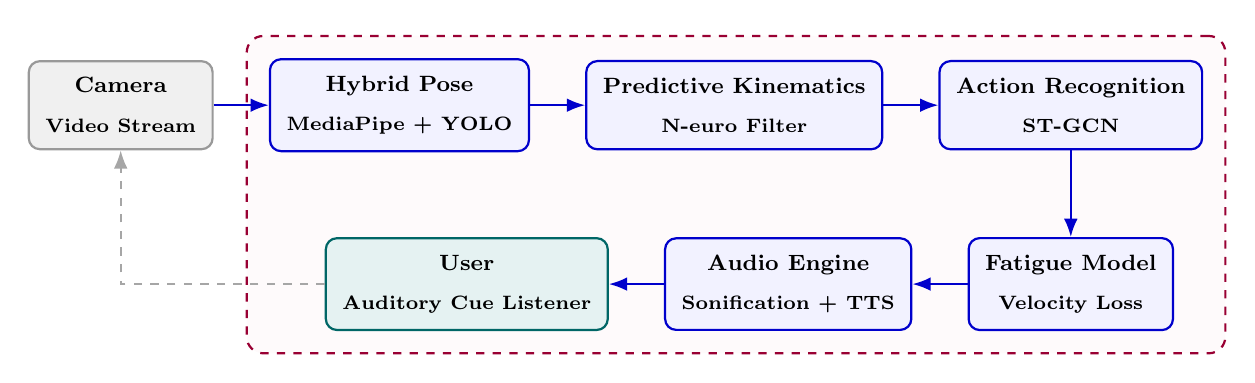
\begin{tikzpicture}[
        node distance=0.6cm and 0.6cm,
        box/.style={rectangle, rounded corners=4pt, draw=blue!80!black, fill=blue!5, thick, align=center, inner sep=6pt, font=\footnotesize\bfseries},
        ext/.style={rectangle, rounded corners=4pt, draw=gray!80, fill=gray!12, thick, align=center, inner sep=6pt, font=\footnotesize\bfseries},
        user/.style={rectangle, rounded corners=4pt, draw=teal!80!black, fill=teal!10, thick, align=center, inner sep=6pt, font=\footnotesize\bfseries},
        pbox/.style={draw=purple!80!black, fill=purple!2, dashed, thick, rounded corners=6pt, inner sep=8pt},
        arr/.style={-Latex, thick, draw=blue!80!black},
        fbarr/.style={-Latex, thick, dashed, draw=gray!70}
    ]
        % Top Row
        \node[ext] (cam) {\textbf{Camera}\\[0.2em]\scriptsize Video Stream};
        \node[box, right=0.7cm of cam] (pose) {\textbf{Hybrid Pose}\\[0.2em]\scriptsize MediaPipe + YOLO};
        \node[box, right=0.7cm of pose] (pred) {\textbf{Predictive Kinematics}\\[0.2em]\scriptsize N-euro Filter};
        \node[box, right=0.7cm of pred] (act) {\textbf{Action Recognition}\\[0.2em]\scriptsize ST-GCN};
        
        % Bottom Row
        \node[box, below=1.1cm of act] (fat) {\textbf{Fatigue Model}\\[0.2em]\scriptsize Velocity Loss};
        \node[box, left=0.7cm of fat] (aud) {\textbf{Audio Engine}\\[0.2em]\scriptsize Sonification + TTS};
        \node[user, left=0.7cm of aud] (usr) {\textbf{User}\\[0.2em]\scriptsize Auditory Cue Listener};
        
        % Surrounding Edge Container
        \begin{scope}[on background layer]
            \node[pbox, fit=(pose) (pred) (act) (fat) (aud), label={[font=\bfseries\scriptsize, text=purple!80!black, yshift=-0.15cm]above:}] (pipe) {};
        \end{scope}
        
        % Connections
        \draw[arr] (cam) -- (pose);
        \draw[arr] (pose) -- (pred);
        \draw[arr] (pred) -- (act);
        \draw[arr] (act) -- (fat);
        \draw[arr] (fat) -- (aud);
        \draw[arr] (aud) -- (usr);
        \draw[fbarr] (usr.west) -| node[near start, below, font=\tiny\bfseries, text=gray!80]{} (cam.south);
    \end{tikzpicture}
    }
    \caption{R.E.A.P System Architecture and Closed-Loop Pipeline}
    \label{fig:architecture}
\end{figure}

The audio feedback module combines continuous sonification (pitch modulations signaling angle boundaries) and local Text-to-Speech (TTS) synthesis, generating verbal cues within $40$\,ms of detected form deviation without external cloud transmission.

% ====================================================Chapter 4===============================================================
\begin{center}
    \justifying
    \chapter{SOFTWARE REQUIREMENTS AND TIMELINE}
\end{center}

\section{Software Requirement Specification}
The software requirements for R.E.A.P are structured into functional and non-functional specifications:

\subsection{Functional Requirements (FR)}
\begin{itemize}[label=$\blacktriangleright$]
    \item \textbf{FR-1: Kinematic Tracking:} Continuously track 33 full-body anatomical landmarks from a monocular video feed, computing joint angles and spatial velocity profiles.
    \item \textbf{FR-2: Deviation Analytics:} Calculate biomechanical deviations against clinically validated pose baselines in real time.
    \item \textbf{FR-3: Real-Time Audio:} Synthesize real-time audio tones and concise TTS corrective prompts instructing proper form.
    \item \textbf{FR-4: Fatigue Profiling:} Track Mean Concentric Velocity (MCV) across repetitions to warn users of impending muscular failure.
\end{itemize}

\subsection{Non-Functional Requirements (NFR)}
\begin{itemize}[label=$\blacktriangleright$]
    \item \textbf{NFR-1: Latency Limits:} End-to-end visual-to-audio latency must not exceed $150$\,ms.
    \item \textbf{NFR-2: Total Localization:} 100\% on-device execution with zero cloud dependency during exercise execution.
    \item \textbf{NFR-3: Audio-First Usability:} Enable completely hands-free and eyes-free workout execution, preserving cervical spine neutrality.
    \item \textbf{NFR-4: System Modularity:} Plug-in Python framework allowing seamless addition of new exercise profiles.
\end{itemize}

Table~\ref{table:srs_summary} summarizes the Software Requirements Specification.

\begin{table}[ht]
    \caption{Software Requirements Specification Summary}
    \label{table:srs_summary}
    \centering
    \small
    \begin{tabularx}{\linewidth}{>{\bfseries}l >{\raggedright\arraybackslash}p{4cm} >{\raggedright\arraybackslash}X}
        \toprule
        \textbf{ID} & \textbf{Requirement Name} & \textbf{Target Specification} \\
        \midrule
        \textbf{FR-1} & Kinematic Tracking & 33 3D Keypoints at $\ge 30$\,FPS \\
        \textbf{FR-2} & Deviation Analytics & Joint angle deviation $< 3^\circ$ tolerance \\
        \textbf{FR-3} & Real-Time Audio & Synthesized corrective prompts $< 150$\,ms \\
        \textbf{FR-4} & Fatigue Profiling & Velocity loss monitoring ($V_{\text{loss}} \ge 20\%$) \\
        \textbf{NFR-1} & End-to-End Latency & $\le 150$\,ms roundtrip \\
        \textbf{NFR-2} & Edge Localization & Zero cloud dependency; 100\% offline \\
        \textbf{NFR-3} & Audio-First Usability & Eyes-free training; cervical neutrality \\
        \textbf{NFR-4} & Modular Extensibility & JSON/Python exercise plugin schema \\
        \bottomrule
    \end{tabularx}
\end{table}

\section{Project Timeline and Milestone Schedule}
The project work is distributed across Semester~7 (Major Project--I) and Semester~8 (Major Project--II). Table~\ref{table:timeline} presents the structured workstream schedule.

\begin{table}[ht]
    \caption{Project Timeline and Workstream Milestones (Semesters 7 \& 8)}
    \label{table:timeline}
    \centering
    \footnotesize
    \begin{tabularx}{\linewidth}{>{\raggedright\arraybackslash}X *{8}{>{\centering\arraybackslash}p{0.8cm}}}
        \toprule
        \multirow{2}{*}{\textbf{Phase / Workstream}} & \multicolumn{4}{c|}{\textbf{Semester 7 (2026)}} & \multicolumn{4}{c}{\textbf{Semester 8 (2027)}} \\
        \cline{2-9}
         & \textbf{Sep} & \textbf{Oct} & \textbf{Nov} & \textbf{Dec} & \textbf{Jan} & \textbf{Feb} & \textbf{Mar} & \textbf{Apr} \\
        \midrule
        Tracking Integration & \cellcolor{blue!30}\textbf{X} & & & & & & & \\
        Core Edge Framework & & \cellcolor{blue!30}\textbf{X} & \cellcolor{blue!30}\textbf{X} & & & & & \\
        Local Audio Engine & & & & \cellcolor{blue!30}\textbf{X} & & & & \\
        Fatigue Modeling & & & & & \cellcolor{blue!30}\textbf{X} & \cellcolor{blue!30}\textbf{X} & & \\
        HCC Older Adults Testing & & & & & & & \cellcolor{blue!30}\textbf{X} & \\
        Algorithm Iteration & & & & & & & & \cellcolor{blue!30}\textbf{X} \\
        \bottomrule
    \end{tabularx}
\end{table}

\noindent \textbf{Phase Descriptions:}
\begin{itemize}
    \item \textbf{Sep 2026 (Completed):} Evaluated MediaPipe and YOLO-Pose baselines; constructed hybrid pose fallback mechanisms.
    \item \textbf{Oct -- Nov 2026 (In Progress):} Setup the modular Python application core and integrated N-euro predictor weights for zero-lag trajectory filtering.
    \item \textbf{Dec 2026:} Develop and benchmark the on-device audio feedback engine for sub-second auditory latency.
    \item \textbf{Jan -- Feb 2027:} Implement Velocity-Based Training analytics and predictive fatigue modeling algorithms.
    \item \textbf{Mar 2027:} Conduct real-world user testing and clinical validation with older adults at Health Care Centers (HCC).
    \item \textbf{Apr 2027:} Perform final algorithmic iterations, ablation studies on ST-GCN and N-euro accuracy, and compile the final B.Tech. dissertation.
\end{itemize}

% ===================================================Chapter 5===============================================================
\begin{center}
    \justifying
    \chapter{CONCLUSIONS AND FUTURE WORK}
\end{center}

\section{Summary of Mid-Semester Evaluation}
In this Major Project--I mid-semester phase, we have systematically established the theoretical, architectural, and initial algorithmic foundations of \textbf{R.E.A.P : Realtime Edge Agentic Physio-Buddy}:
\begin{enumerate}[label=\textbf{(\arabic*)}]
    \item \textbf{Market and Clinical Gap Analysis:} Investigated existing solutions (QuickPose, Kemtai, Metric VBT), isolating three fundamental drawbacks: latency compromises from heuristic filtering, cloud privacy vulnerabilities, and neck strain induced by screen-based interfaces.
    \item \textbf{Kinematic Engine Prototyping:} Successfully integrated an ensemble pose estimation pipeline combining MediaPipe BlazePose and YOLO-Pose, achieving reliable joint landmark tracking in varying home environments.
    \item \textbf{Predictive Trajectory Formulation:} Analyzed and implemented the N-euro Predictor mathematical framework to overcome the classical 1-Euro jitter-lag tradeoff.
    \item \textbf{Kinetic Chain and SRS Formalization:} Formulated the ST-GCN graph topology for full-body kinematic analysis and finalized the comprehensive Software Requirement Specification.
\end{enumerate}

\section{Work in Progress and Semester 8 Roadmap}
The trajectory for the remainder of Major Project--I and Major Project--II comprises the following milestones:
\begin{itemize}[label=$\blacktriangleright$]
    \item \textbf{Hardware Optimization:} Quantize the ST-GCN and N-euro neural network weights using INT8 precision to ensure execution under $150$\,ms on mobile Neural Processing Units (NPUs).
    \item \textbf{Audio Sonification Refinement:} Calibrate acoustic feedback frequencies with sports physiotherapists to ensure that auditory cues are intuitive, unambiguous, and non-intrusive.
    \item \textbf{Clinical Testing in HCC:} Partner with local Health Care Centers (HCC) to conduct empirical usability and injury-prevention trials with older adults performing guided mobility routines.
    \item \textbf{Dissertation and Publication:} Perform extensive ablation studies comparing R.E.A.P against traditional heuristic filters and compile findings into the final dissertation.
\end{itemize}

% ==============================================================================
% REFERENCES
% ==============================================================================
\begin{thebibliography}{99}

\bibitem{li2018stgcn}
C.~Li, Z.~Cui, W.~Zheng, C.~Xu, and J.~Yang,
\newblock ``Spatio-temporal graph convolution for skeleton based action recognition,''
\newblock in \emph{Proceedings of the AAAI Conference on Artificial Intelligence}, vol.~32, no.~1, 2018. \url{https://doi.org/10.1609/aaai.v32i1.11776}

\bibitem{shao2023neuro}
Q.~Shao, J.~Wang, B.~Zhou, V.~A.~Tran, G.~Krishnan, and S.~Nayar,
\newblock ``N-euro predictor: A neural network approach for smoothing and predicting motion trajectory,''
\newblock \emph{Proceedings of the ACM on Interactive, Mobile, Wearable and Ubiquitous Technologies (IMWUT/UbiComp)}, vol.~7, no.~1, pp. 1--25, 2023. \url{https://doi.org/10.1145/3610884}

\bibitem{yan2018spatial}
S.~Yan, Y.~Xiong, and D.~Lin,
\newblock ``Spatial temporal graph convolutional networks for skeleton-based action recognition,''
\newblock in \emph{Thirty-Second AAAI Conference on Artificial Intelligence}, 2018.

\bibitem{casiez2012euro}
G.~Casiez, N.~Roussel, and D.~Vogel,
\newblock ``1-Euro filter: a simple speed-based low-pass filter for noisy input in human-computer interaction,''
\newblock in \emph{Proceedings of the SIGCHI Conference on Human Factors in Computing Systems}, pp. 2527--2530, 2012.

\bibitem{sanchez2011velocity}
L.~S{\'a}nchez-Medina and J.~J.~Gonz{\'a}lez-Badillo,
\newblock ``Velocity loss as an indicator of neuromuscular fatigue during resistance training,''
\newblock \emph{Medicine \& Science in Sports \& Exercise}, vol.~43, no.~9, pp. 1725--1734, 2011.

\end{thebibliography}

\end{document}
